\subsection{Continuous Solids and the Common Analyzed Domain}
For mechanical time $t_m$, let $A_k(t_m)$ be the padded analyzed interior of layer $k$. The lateral domain is their intersection, not the intersection of their voids:
\begin{equation}
A_\cap(t_m)=\bigcap_{k=1}^{N_z}A_k(t_m),\qquad
\mathcal A=A_\cap\times[0,L_z].
\label{eq:common-domain}
\end{equation}
Each backbone and cohesive segment is represented by a planar capsule of radius $r_f$, and each platelet by a disk of radius $r_p$. These primitives are extruded over the corresponding layer slab; their union is the solid $\mathcal S$. Cohesive links have the same geometric radius as backbone segments. The construction approximates a multilayer material; it does not impose mechanical coupling between planes or reconstruct spherical platelets and curved fibers in three dimensions.

The common lateral boundary retains the native $256\times256$ support raster, with spacing approximately $0.186~\mu\mathrm m$. It is an artificial reflecting boundary for tracer centers and is not eroded again by the tracer radius. Solid exclusion instead uses continuous center-to-solid distance. For tracer radius $a_{\rm tr}$,
\begin{equation}
\begin{aligned}
\mathcal V&=\mathcal A\setminus\mathcal S,\\
\Omega_{\rm acc}&=\{\mathbf r\in\mathcal A:
\operatorname{dist}(\mathbf r,\mathcal S)\ge a_{\rm tr}\}.
\end{aligned}
\label{eq:accessible-centers}
\end{equation}
Finite-particle clearance applies to the internal solid. Escape is defined by the center reaching either external $z$ face, not by complete clearance of the sphere beyond that face.

\section{Configuration and Structure--Transport Observables}
Nine mechanical seed blocks generate paired force conditions $f_0=0$, 2.2, 4.4, and 8.8 nN. Each stack contains 50 independently generated planes with $H=100$ nm, giving $L_z=N_zH=5~\mu\mathrm m$. Frozen snapshots at $t_m=0$, 5, 10, and 15 s are analyzed. There are 144 condition labels but 117 unique geometries, because the four forces share the same initial state within each seed block. Figure~\ref{fig1} shows the mechanical evolution of layer 1 from replica 1 at $f_0=2.2$ nN.

Figure~\ref{fig:solid-stack-current} illustrates the assembly of independent mechanical planes into the solid stack used to define tracer exclusion. The display voxelization does not replace the continuous primitives used for transport.

\begin{figure}[tbp]
\centering
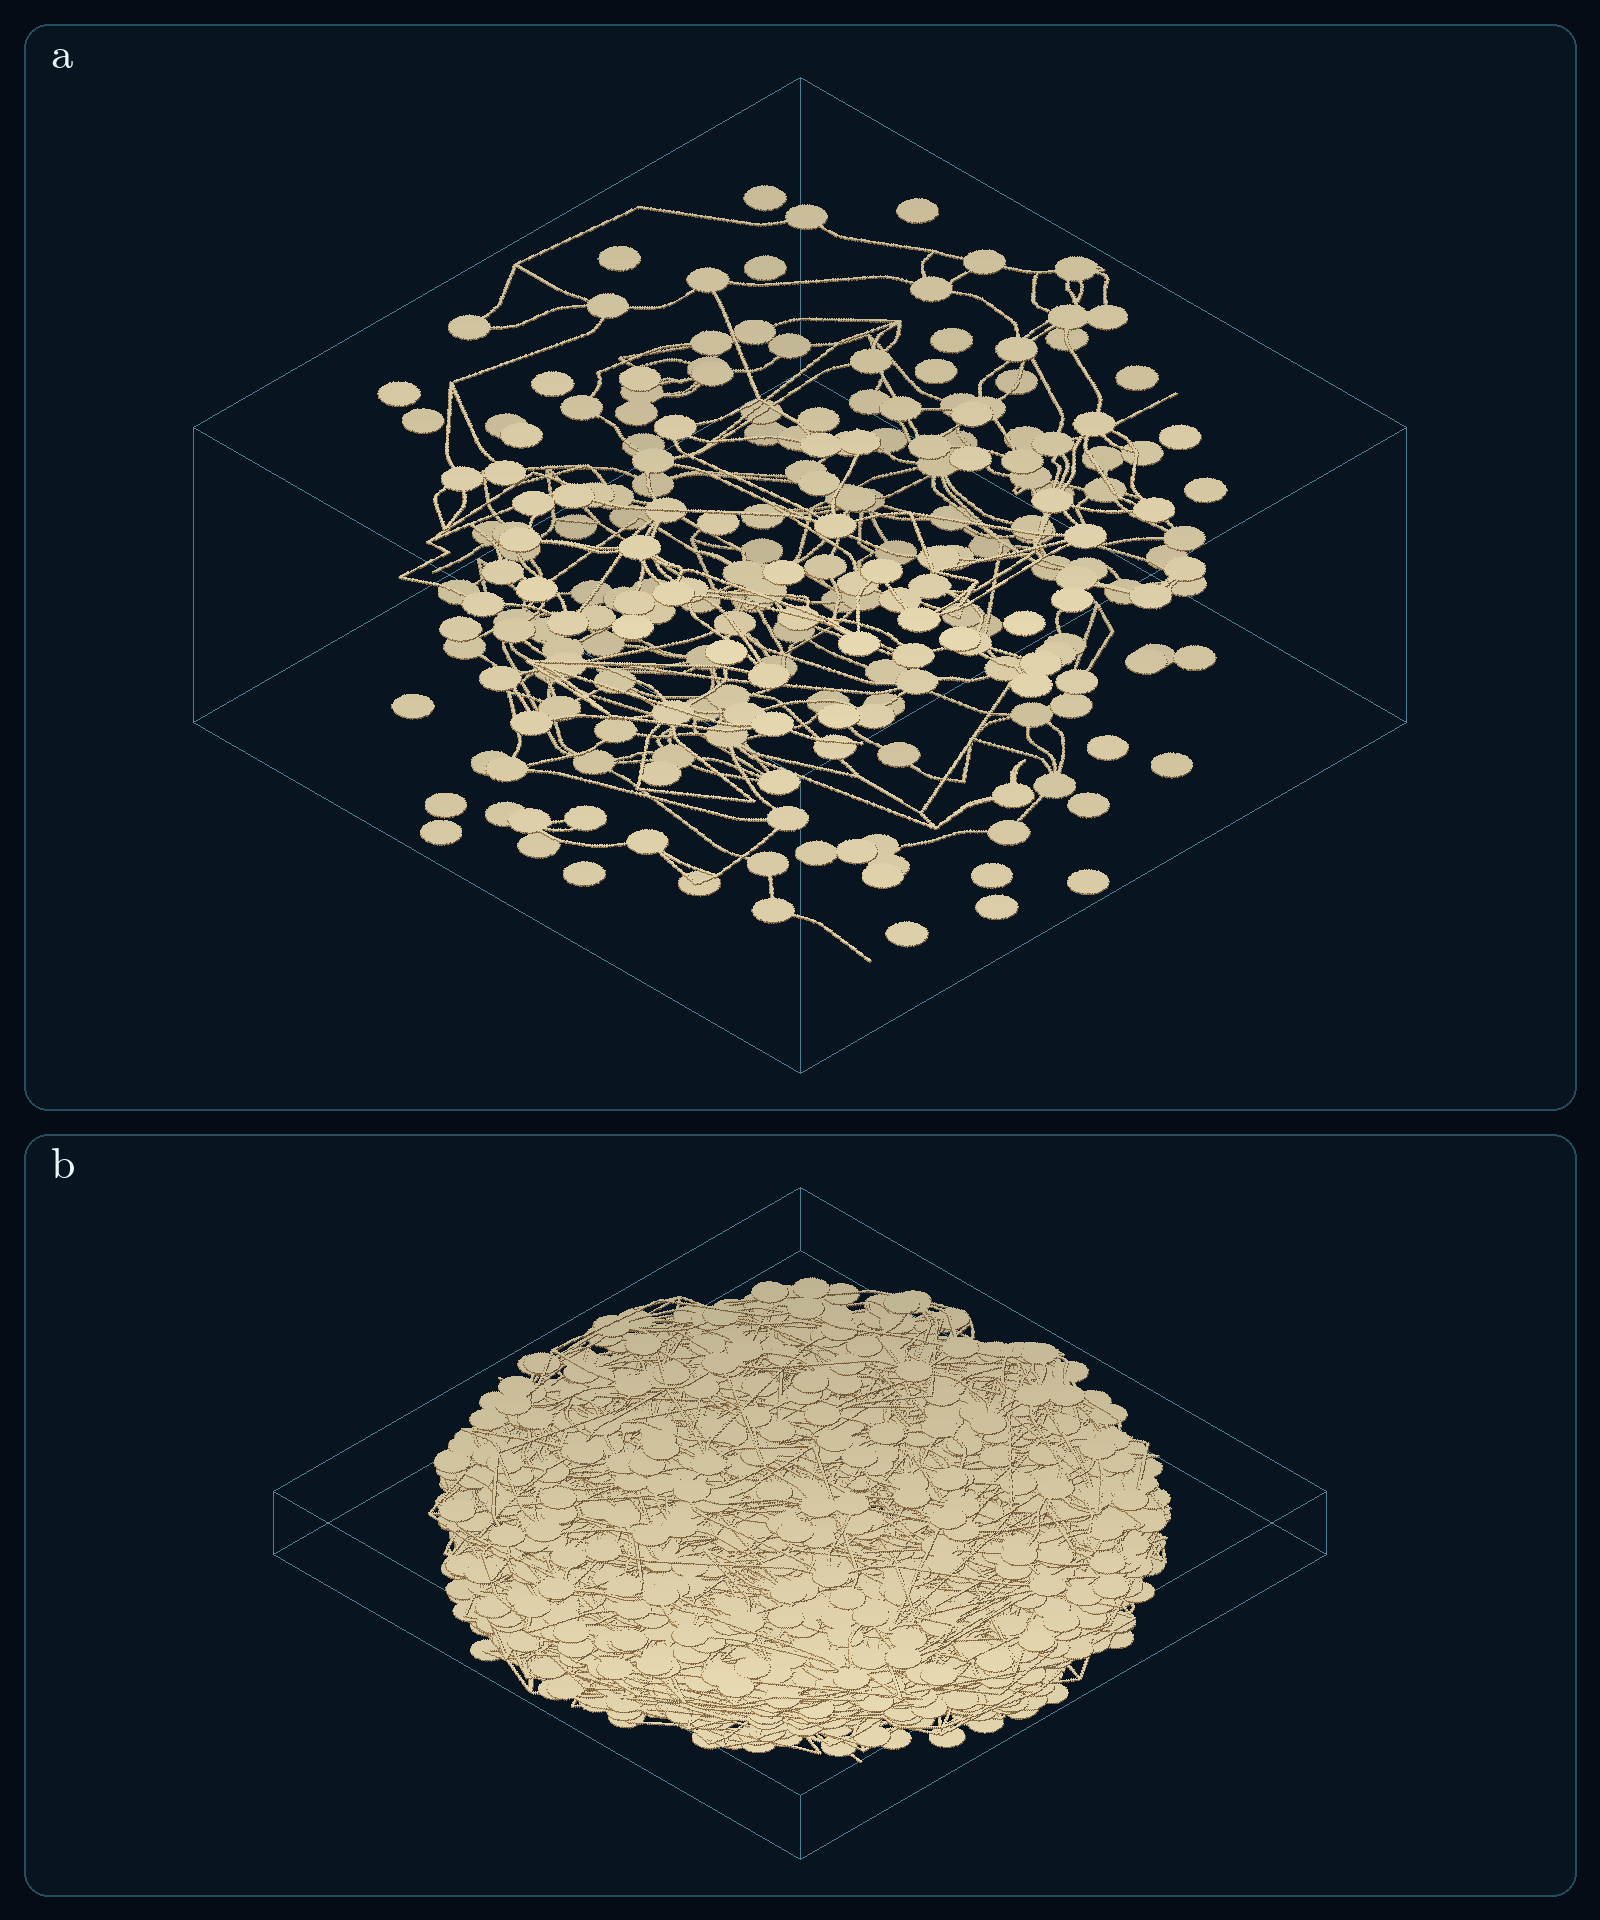
\includegraphics[width=\linewidth]{figures/figure_solid_50layer.png}
\caption{Solid assembly from replica 1 at $f_0=2.2$ nN and $t_m=10$ s. (a) Layers 1, 13, 25, 37, and 50, with separation expanded for display. (b) All 50 layers at $H=100$ nm ($L_z=5~\mu\mathrm m$), without axial exaggeration. Fibrin, cohesive links, and platelets share one opaque color. Voxels approximate the continuous solids for display only; the full lateral field is shown, without clipping to the common analyzed boundary.}
\label{fig:solid-stack-current}
\end{figure}

\subsection{Contraction, Accessibility, and Initial Connectivity}
\label{sec:structural-readouts}
Mechanical time $t_m$ selects a saved network configuration; transport time $t$ starts at tracer release and advances while that configuration remains fixed. Projected-area contraction assays motivate normalization by the initial area \cite{Prakhya2022}. We distinguish the layer-mean and common-domain measures:
\begin{equation}
\begin{aligned}
C_{A,\rm layer}(t_m)&=1-\frac{\overline{|A_k(t_m)|}}{\overline{|A_k(0)|}},\\
C_{A,\cap}(t_m)&=1-\frac{|A_\cap(t_m)|}{|A_\cap(0)|}.
\end{aligned}
\label{eq:area-contraction}
\end{equation}
Here $|A|$ denotes the area of a planar region, and $\overline{|A_k(t_m)|}=N_z^{-1}\sum_{k=1}^{N_z}|A_k(t_m)|$ is the mean area across layers.
Both characterize computationally defined projected regions, not solid-volume loss or volumetric strain. The paired results below use $C_{A,\cap}$; the layer-mean values remain in the data archive.

For the same geometry and tracer radius,
\begin{equation}
\phi_{\rm acc}=\frac{|\Omega_{\rm acc}|}{|\mathcal A|},
\qquad V_{\rm acc}=\phi_{\rm acc}|\mathcal A|.
\label{eq:accessible-fraction}
\end{equation}
Absolute accessible volume is reported alongside the fraction because contraction changes the denominator. Clearance is sampled using 131072 uniform box proposals per mechanical replica, shared across its states and restricted to the common domain. Accessibility includes valid centers in isolated components; it is not itself an escape probability.

Let $\Omega_{\rm exit}$ contain accessible centers connected to at least one absorbing $z$ face. For the $N_0$ actual starting centers, the target quantity is
\begin{equation}
\widehat F_{\rm conn}=\frac1{N_0}\sum_i
\mathbf1\{\mathbf R_i(0)\in\Omega_{\rm exit}\}.
\label{eq:initial-connectivity}
\end{equation}
Connection to both faces is unnecessary for central-release escape. Connectivity is assessed independently of the observed trajectories using conservative inner and outer cell graphs and checked continuous bridges. With $n_+$ connected, $n_-$ disconnected, and $n_?$ unresolved starts, the resulting bounds are
\begin{equation}
\frac{n_+}{N_0}\le\widehat F_{\rm conn}
\le1-\frac{n_-}{N_0}.
\label{eq:connectivity-bounds}
\end{equation}
A missing certified path does not establish isolation. Details of the auxiliary grid and bridge search are given in Supplementary Sec.~S8.

\subsection{Central Release and Reflecting Tracer Transport}
\label{sec:tracer-transport}
Each unique geometry uses 256 noninteracting spherical tracers with $a_{\rm tr}=0.25~\mu\mathrm m$ and $D=0.4~\mu\mathrm m^2\mathrm s^{-1}$. The diameter is compatible with a circulating-microparticle size scale \cite{Zubairova2015}; the diffusion coefficient is an assumed effective parameter, not measured or calibrated to that paper. Initial centers are sampled in a central cylinder of radius $1.19~\mu\mathrm m$ with $2\le z\le3~\mu\mathrm m$, conditioned on solid clearance but not exit connectivity (Fig.~\ref{fig:tracer-initialization}).

\begin{figure}[tbp]
\centering
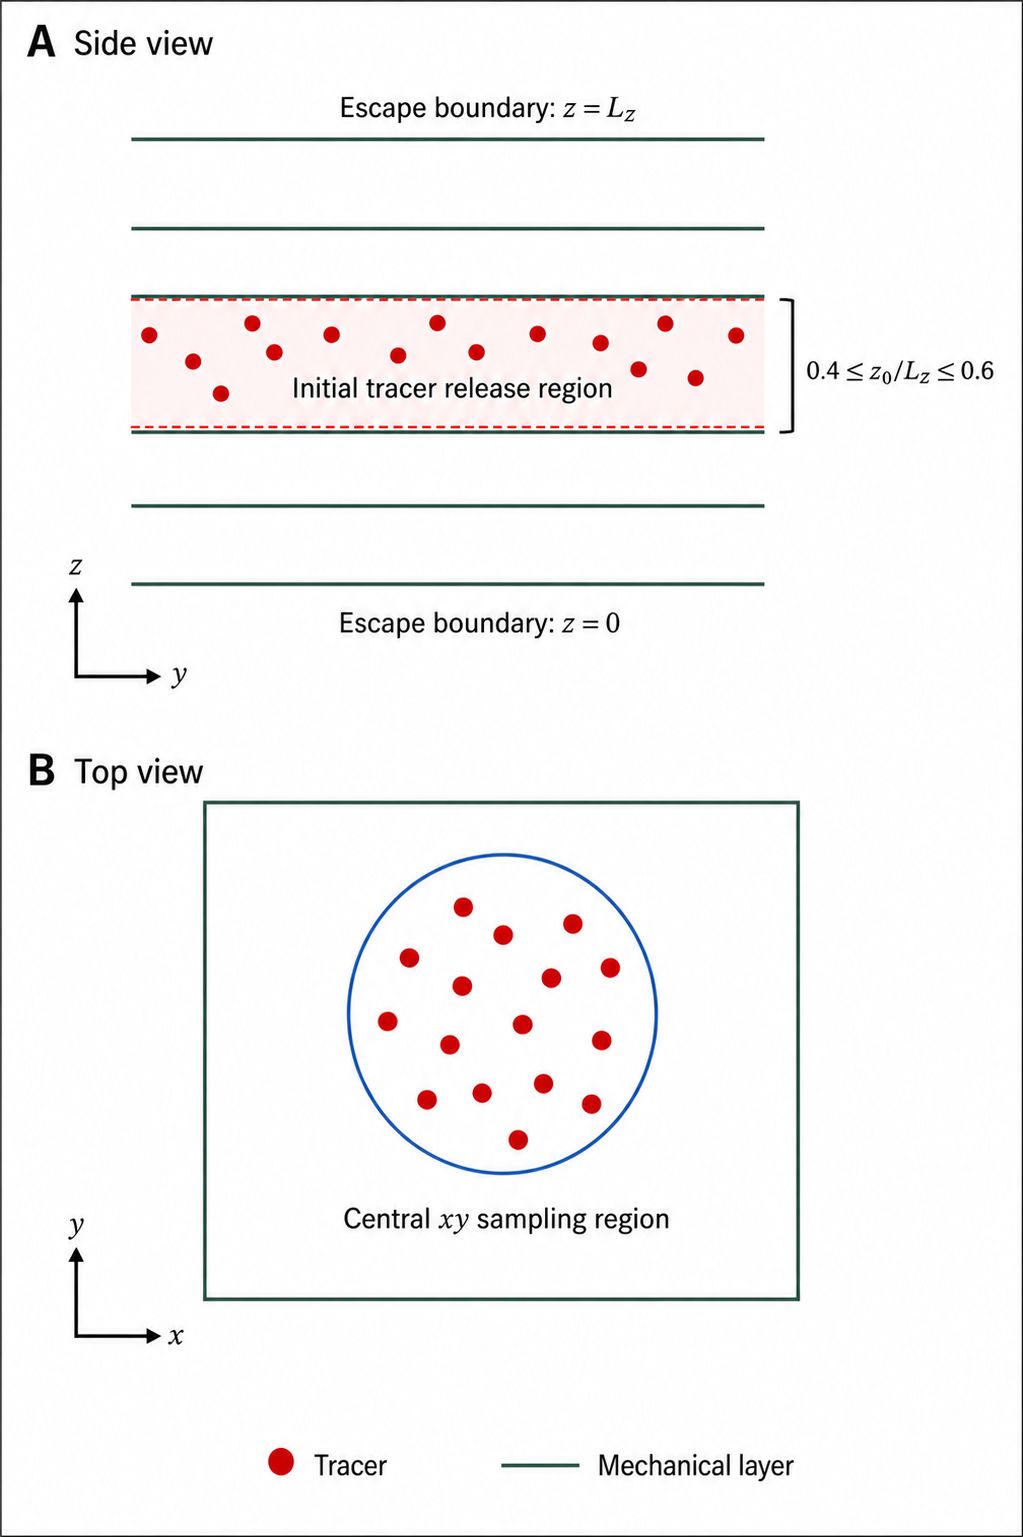
\includegraphics[width=\linewidth]{figures/tracer_initial_condition_vertical.png}
\caption{Central release in the band $0.4\le z_0/L_z\le0.6$. The lateral sampling disk has radius $1.19~\mu\mathrm m$. Escape occurs when the center first reaches $z=0$ or $z=L_z$; the analyzed lateral boundary reflects.}
\label{fig:tracer-initialization}
\end{figure}

The free proposal is
\begin{equation}
\Delta\mathbf R=\sqrt{2D\Delta t}\,\boldsymbol\eta,
\qquad\boldsymbol\eta\sim\mathcal N(\mathbf0,I_3),
\label{eq:tracer-transport}
\end{equation}
with $\Delta t=0.015625$ ms. The swept segment is checked for the first contact with the radius-expanded solid or lateral boundary. At a smooth contact with unit normal $\mathbf n$, the remaining displacement is reflected:
\begin{equation}
\Delta\mathbf R_{\rm rem}'=\Delta\mathbf R_{\rm rem}
-2(\Delta\mathbf R_{\rm rem}\cdot\mathbf n)\mathbf n.
\label{eq:reflection}
\end{equation}
Further contacts are resolved within the same increment. Simultaneous independent normals define a reflected normal subspace; a tied obstacle contact is processed before an axial exit. Geometric subdivision accommodates long sequences of reflections without resampling noise or changing physical time. Failures stop execution rather than being recorded as censoring.

This is a drift-free geometric reflection scheme, not the general force-dependent transition-probability algorithm of Behringer and Eichhorn \cite{BehringerEichhorn2012}. Its planar-wall behavior follows the image construction, whereas curved boundaries, repeated contacts, and exit timing retain finite-step error. The primary exit time is the step endpoint; a separately saved linear crossing time is not treated as an exact Brownian first-passage time.

\subsection{Survival and Restricted Mean Exit Time}
Let $\tau$ be the first time the tracer reaches either axial face. Survival is $S(t)=\Pr(\tau>t)$ \cite{Redner2001}. All histories end at escape or the common administrative horizon $T_c=100$ s, so
\begin{equation}
\widehat S(t)=1-\frac{N_{\rm escape}(t)}{N_0},
\qquad 0\le t\le T_c.
\label{eq:survival-probability}
\end{equation}
The restricted mean first-passage time is
\begin{equation}
\begin{aligned}
\widehat{\mathrm{RMST}}(T_c)
&=\frac1{N_0}\sum_i\min(\tau_i,T_c)\\
&=\int_0^{T_c}\widehat S(t)\,\mathrm dt.
\end{aligned}
\label{eq:restricted-met}
\end{equation}
Each censored history contributes $T_c$; averaging only escaped histories would estimate a different, selected quantity. The general restricted-time definition \cite{RoystonParmar2013} requires no clinical hazard model here. Finite-time survival does not demonstrate adhesion or permanent capture.

For a fixed domain and a fully resolved initial connected fraction $F_{\rm conn}$, partitioning the initial population gives
\begin{equation}
S(t)=1-F_{\rm conn}+F_{\rm conn}S_{\rm conn}(t),
\label{eq:survival-connectivity}
\end{equation}
and
\begin{equation}
\begin{aligned}
\mathrm{RMST}(T_c)={}&(1-F_{\rm conn})T_c\\
&+F_{\rm conn}\mathrm{RMST}_{\rm conn}(T_c).
\end{aligned}
\label{eq:rmst-connectivity}
\end{equation}
These identities distinguish loss of routes from slow motion in connected space. They cannot be numerically decomposed using unresolved connectivity bounds as if those bounds were exact fractions.

\subsection{Paired Comparisons and Uncertainty}
\label{sec:comparison-framework}
For an observable $Y$, each active-baseline state is compared with its own zero-baseline control at the same mechanical time:
\begin{equation}
\Delta Y_r(f_0,t_m)=Y_r(f_0,t_m)-Y_r(0,t_m).
\label{eq:paired-change}
\end{equation}
Here $r$ identifies a mechanical seed block. The control retains stiffness-dependent filopodial traction, as specified by Eq.~\eqref{eq:wlctraction}; it is not an inactive-platelet condition. Changes from the initial snapshot are stored separately.

Initial proposal pools and per-particle Gaussian seeds are reused within each replica. Validity filtering changes accepted starting coordinates: force-control pairs share 26--225 of 256 physical positions, often at different indices, and at most 68 at identical indices. Thus pairing does not imply identical physical starts. The initial population is native to each geometry and is never filtered by subsequent escape.

Transport contrasts use 10000 percentile-bootstrap resamples of paired particle indices \cite{Efron1979}. The 95\% intervals are approximate, marginal, and conditional on the chosen networks and observed starting samples. They do not provide simultaneous coverage, full uncertainty propagation through initial sampling, between-network uncertainty, or numerical error bounds. Geometry and transport contrasts retain the nine mechanical replicas separately; mean survival curves are accompanied by their minimum--maximum range. No population-level significance claim is based on 256 tracers or 50 layers as if they were independent clots. Comparisons between the 15 and 10 s mechanical states use the same paired-index procedure and remain conditional on the two accepted starting samples.

\subsection{Numerical Verification and Scope}
\label{sec:verification}
Implementation checks, analytical references, and sensitivity studies answer different questions. The supplement preserves the fixed-mask and cropped continuous-geometry studies with their original boundary rules. Their conditional conclusions are not transferred to the present reflecting, cohesion-inclusive full common domain.

The reflecting implementation passed 26510 geometric and propagation cases, including analytic first contacts, independent segment--box comparisons, planar images, and multiple-reflection controls. A larger-sample temporal study compares $\Delta t=0.03125$, 0.015625, and 0.0078125 ms until $T_c=100$ s, using 8192 paired histories per step in each of three frozen states: replica 1 at 0 s, replica 1 at $f_0=2.2$ nN and 10 s, and replica 9 at $f_0=8.8$ nN and 15 s. These are three states from two mechanical seed groups. Initial positions are identical across steps within a state, and coarse Brownian increments sum the finer increments. Independent new tracer seeds distinguish these 73728 verification histories from the 29952 production histories.

For the primary comparison, 0.015625 minus 0.0078125 ms, all three relative RMST intervals meet the $\pm3\%$ tolerance. Survival differences are $0.024$, $0.806$, and $-0.049$ pp, with marginal 97.5\% intervals $[-1.398,1.447]$, $[-0.782,2.392]$, and $[-1.424,1.326]$ pp. All meet the revised operational margin of $\pm2.5$ pp. This survival margin was revised after examining the results; the originally fixed $\pm2$ pp margin remains inconclusive for the intermediate state. Thus the selected 0.015625 ms step satisfies practical equivalence under the revised criterion in the tested states, not a successful confirmation of the original criterion \cite{Lakens2017}. Neither the revision nor the refinement changes the production trajectories. The full intervals, their construction, and the initial 256-history comparison are retained in Supplement S8. This evidence does not establish uniform survival-curve equivalence, every-state temporal convergence, or spatial transport convergence.

\section{Results: Homogeneous Frozen-State Pilot}
The cohort contains nine paired mechanical seed blocks per force. Block 1 uses layer seeds 4000--4019 and 4040--4069; block 2 uses 4020--4039 and 4070--4099. Blocks 3--9 use consecutive groups of 50 seeds from 4100--4149 through 4400--4449. Each force reuses these blocks. There are 29952 unique tracer histories over 117 geometries. The cohort was extended sequentially: 13824 completed histories in blocks 1--6 at 0, 5, and 10 s were retained, and 16128 histories cover blocks 7--9 at those times and all nine blocks at 15 s. The per-state allocation of 256 histories was fixed before analyzing each batch, without outcome-dependent trajectory stopping.

\begin{table*}[t]
\centering\footnotesize
\setlength{\tabcolsep}{3.4pt}
\caption{Homogeneous frozen-state pilot. Values are means across nine paired mechanical replicas; bracketed transport ranges are minimum--maximum, not confidence intervals. Each unique geometry has 256 histories, tracer diameter $0.50~\mu\mathrm m$, $D=0.4~\mu\mathrm m^2/\mathrm s$, and $T_c=100$ s. The shared initial state is listed once. Contraction refers to the common analyzed region.}
\label{tab:homogeneous-pilot}
\begin{tabular}{@{}rrrrcc@{}}
\toprule
$t_m$ (s) & $f_0$ (nN) & $C_{A,\cap}$ (\%) & $\phi_{\rm acc}$ (\%) & $S(100)$ (\%) & RMST(100) (s) \\ \midrule
0 & all & 0.000 & 15.322 & $24.22\ [12.11,53.12]$ & $55.97\ [43.53,76.40]$ \\
\specialrule{0.2pt}{1.5pt}{1.5pt}
5 & 0 & 0.034 & 15.375 & $25.48\ [10.55,55.86]$ & $56.23\ [42.51,76.58]$ \\
\specialrule{0.2pt}{1.5pt}{1.5pt}
5 & 2.2 & 1.112 & 17.180 & $21.35\ [10.94,41.02]$ & $51.63\ [41.55,69.39]$ \\
\specialrule{0.2pt}{1.5pt}{1.5pt}
5 & 4.4 & 1.725 & 17.929 & $17.53\ [4.69,29.30]$ & $50.04\ [40.04,61.34]$ \\
\specialrule{0.2pt}{1.5pt}{1.5pt}
5 & 8.8 & 2.466 & 18.610 & $18.01\ [9.77,27.73]$ & $48.74\ [36.76,62.34]$ \\
\specialrule{0.2pt}{1.5pt}{1.5pt}
10 & 0 & 0.064 & 15.436 & $27.08\ [14.06,60.55]$ & $56.91\ [44.65,78.36]$ \\
\specialrule{0.2pt}{1.5pt}{1.5pt}
10 & 2.2 & 1.845 & 17.979 & $19.92\ [12.11,29.69]$ & $50.56\ [41.76,61.81]$ \\
\specialrule{0.2pt}{1.5pt}{1.5pt}
10 & 4.4 & 2.727 & 18.806 & $18.45\ [8.20,34.77]$ & $48.82\ [36.58,66.03]$ \\
\specialrule{0.2pt}{1.5pt}{1.5pt}
10 & 8.8 & 3.586 & 19.517 & $15.54\ [6.25,29.69]$ & $45.57\ [33.20,57.33]$ \\
\specialrule{0.2pt}{1.5pt}{1.5pt}
15 & 0 & 0.128 & 15.548 & $27.34\ [17.19,55.86]$ & $56.47\ [45.46,76.39]$ \\
\specialrule{0.2pt}{1.5pt}{1.5pt}
15 & 2.2 & 2.426 & 18.531 & $18.53\ [9.38,32.81]$ & $49.69\ [38.32,66.49]$ \\
\specialrule{0.2pt}{1.5pt}{1.5pt}
15 & 4.4 & 3.649 & 19.512 & $16.97\ [7.81,39.06]$ & $47.46\ [35.54,67.27]$ \\
\specialrule{0.2pt}{1.5pt}{1.5pt}
15 & 8.8 & 4.602 & 20.116 & $14.32\ [6.25,29.69]$ & $43.97\ [32.27,59.03]$ \\
\bottomrule
\end{tabular}
\end{table*}


\subsection{Geometric Reorganization}
Figure~\ref{fig:homogeneous-geometry} shows the geometric response of each mechanical replica at 15 s.
In all 81 active-baseline versus zero-baseline contrasts at 5, 10, and 15 s, both common-domain contraction and accessible-center fraction increased. Absolute accessible volume increased by 9.29--27.58\% relative to the matched control, so the fractional change is not merely a shrinking-denominator effect. At 15 s, mean $C_{A,\cap}$ rises from 0.128\% at $f_0=0$ to 4.602\% at 8.8 nN, while mean accessibility rises from 15.548\% to 20.116\% (Table~\ref{tab:homogeneous-pilot}). These are model-geometry estimates, not measurements of a real clot.

\begin{figure}[tbp]
\centering
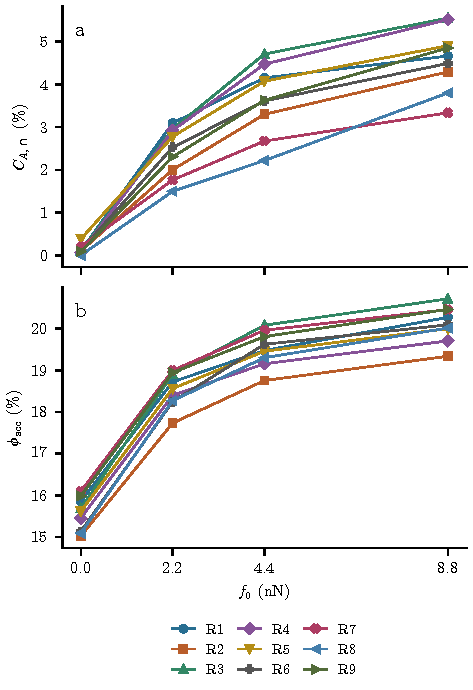
\includegraphics[width=\linewidth]{figures/homogeneous_geometry_tm15.pdf}
\caption{Frozen 15 s geometry: (a) contraction of the common analyzed area and (b) accessible-center fraction. Symbols distinguish the nine paired mechanical replicas. Lines guide the eye; no fitted dose--response law is implied.}
\label{fig:homogeneous-geometry}
\end{figure}

\subsection{Escape and Between-Realization Heterogeneity}
Figure~\ref{fig:homogeneous-transport} compares survival curves and within-replica RMST contrasts at 15 s. Replica-mean survival at 100 s decreases from 27.34\% to 14.32\% between $f_0=0$ and 8.8 nN, while RMST decreases from 56.47 to 43.97 s. Of the 27 active-control contrasts at this mechanical time, 25 have negative RMST point estimates and 21 have conditional intervals entirely below zero. At 8.8 nN, the nine within-replica reductions range from 3.59 to 20.70 s; only the interval for replica 9 includes zero. Replica 9 also has small positive point contrasts at 2.2 and 4.4 nN, and replica 6 has greater RMST at 8.8 than at 4.4 nN despite remaining below its control. The ordering of the aggregate means is therefore not a universal monotonic response.

For example, at 10 s and 4.4 nN, accessible fraction increases by 3.21 pp in replica 1 and 3.02 pp in replica 2, but the RMST changes are $+1.43$ and $-14.04$ s, respectively. Global accessibility alone therefore does not determine the observed residence time. The zero-baseline state of replica 4 at 10 s has $S(100)=60.55\%$ and RMST $=78.36$ s. This realization is retained in the means and ranges, rather than discarded as an outlier. Differences contain both network heterogeneity and conditional tracer-sampling noise; nine replicas do not by themselves establish a general force-effect claim.

\begin{figure}[tbp]
\centering
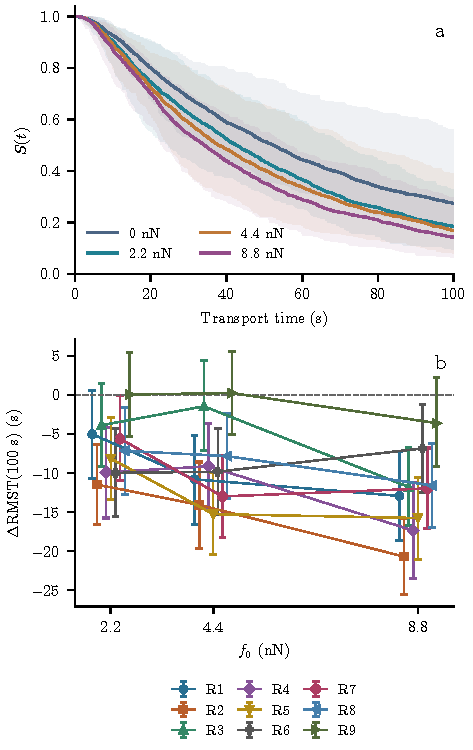
\includegraphics[width=\linewidth]{figures/homogeneous_transport_tm15.pdf}
\caption{Frozen 15 s transport. (a) Mean survival across nine replicas; shading spans their minimum--maximum range, not a confidence interval. (b) Individual-replica RMST differences from the matched $f_0=0$ control, with approximate 95\% conditional bootstrap intervals. These bars do not represent between-clot uncertainty.}
\label{fig:homogeneous-transport}
\end{figure}

Two of 29952 histories contacted the artificial lateral wall: one in replica 8 at 2.2 nN and 10 s (981 contacts), and one in replica 8 at 8.8 nN and 15 s (73 contacts). Direct lateral reflections are therefore rare at the population level, although repeated contacts can occur in an individual history. This count does not exclude effects of the domain definition on geometry or release conditioning. The absorbing-face separation remains 5 $\mu$m; rearrangement does not shorten that axial separation.

\subsection{Comparison Across Frozen Mechanical Times}
Figure~\ref{fig:homogeneous-time} separates the saved mechanical time from the subsequent 100 s transport experiment. With the same nine replicas, advancing the mechanical state from 10 to 15 s changes mean RMST by $-0.44$, $-0.87$, $-1.36$, and $-1.59$ s at baselines 0, 2.2, 4.4, and 8.8 nN, respectively. At the highest baseline, mean $S(100)$ decreases from 15.54\% to 14.32\%, while mean common-area contraction increases from 3.586\% to 4.602\%.

The modest aggregate shifts do not imply uniformly faster escape with further mechanical evolution. Among the 27 active-baseline 15-minus-10 s comparisons, only 14 have negative RMST point differences and five have conditional intervals entirely below zero. Point differences span $-9.08$ to $+4.68$ s. These are comparisons of newly released populations in two frozen geometries, not trajectories followed through a moving network.

\begin{figure}[tbp]
\centering
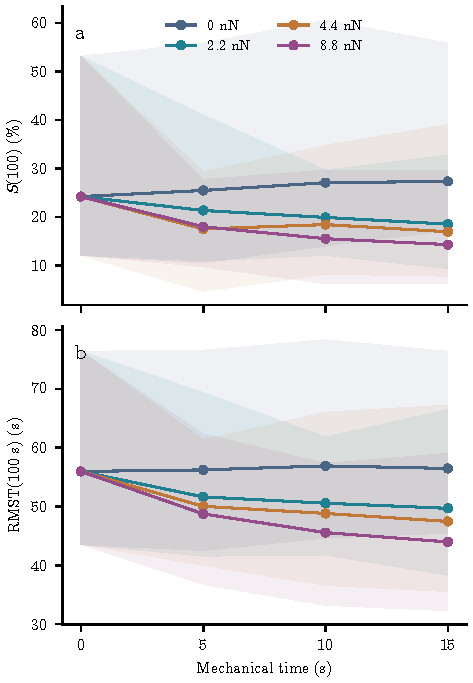
\includegraphics[width=\linewidth]{figures/homogeneous_time_evolution.pdf}
\caption{Frozen-state readouts versus mechanical time: (a) survival at 100 s and (b) RMST restricted to 100 s. Points are means over the same nine replicas; bands span their minimum--maximum range, not confidence intervals. The initial state is shared across forces.}
\label{fig:homogeneous-time}
\end{figure}

\subsection{Connectivity and Finite-Time Retention}
Independent classification certified 20052 connected starts and six disconnected state-specific starts, leaving 9894 unresolved. These are bookkeeping totals across unique conditions, not independent mechanical replicates. Of 6100 histories censored at 100 s, 3380 began at certified connected centers, six at disconnected centers, and 2714 at unresolved centers.

In replica 1 at $f_0=2.2$ nN and $t_m=10$ s, 255 of 256 starts were certified connected. All 64 censored histories belonged to that connected group: their finite-time retention cannot be attributed to an isolated compartment in the specified geometry. Conversely, replica 1 at 4.4 and 8.8 nN and 10 s left all 256 starts unresolved, despite 184 and 205 observed escapes. A zero lower connectivity bound is not zero actual connectivity.

Replica 4 contains one certified disconnected start at 4.4 nN and two at 8.8 nN at 10 s, and one at 2.2 nN and two at 4.4 nN at 15 s. None escaped by 100 s, providing a small non-vacuous consistency check. These six state-specific classifications involve two distinct starting coordinates reused across geometries, not six distinct isolated pores. The wide independent connectivity bounds do not identify the isolated fraction precisely or explain most censored histories.

\section{Discussion}
The supported finding is a separation between geometric accommodation and escape kinetics. Increasing the filopodial baseline produced more projected contraction and accessible volume in all nine seed blocks, but did not produce the same RMST response in each realization. At the highest baseline and 15 s, all nine point estimates favor lower restricted residence, while responses at lower baselines remain heterogeneous. Further evolution from 10 to 15 s yields smaller mean shifts and mixed realization-level changes. Larger accessible volume can coexist with a slowly escaping central population. Certified-connected censored histories demonstrate this distinction; the few certified disconnected starts establish that isolation also occurs in the model without showing that it dominates retention.

The comparison remains exploratory for three reasons. First, nine independent mechanical seed groups show substantial between-realization heterogeneity, and the reported conditional intervals do not establish population-level robustness. Second, the accepted initial distribution changes with geometry, so route changes are not isolated from changes in valid release positions. Third, temporal support is conditional on three tested states and a survival tolerance revised after analysis, while parts of the connectivity classification remain unresolved. Additional mechanical replicas do not themselves resolve numerical error. The revised practical acceptance does not provide numerical bounds for every state or replace external validation.

The construction uses independent mechanical planes and an imposed slab thickness, not a mechanically connected 3D reconstruction. Taking $H=100$ nm equal to the nominal fiber diameter is a modeling choice, not an experimentally established interlayer spacing. The common lateral region and reflecting convention define the analyzed domain; they should not be identified with the exterior of a biological clot. No flow, adhesion, tracer--tracer interaction, permeability, or binding kinetics is modeled. Neither a Brinkman length nor an independent aggregation rate is inferred from these escape histories. Hydraulic tortuosity concerns fluid streamlines \cite{Duda2011} and is not equated to the present restricted residence time.

The free-interval result $u(z)=z(L_z-z)/(2D)$ \cite[Chap.~2]{Redner2001} explains why prescribed thickness and initial axial position matter. A midpoint value $L_z^2/(8D)$ is a useful reference, but it is not an exact normalization for a clearance-conditioned band of starts or a censored observation. We therefore retain $S(t)$ and RMST as the primary transport readouts rather than reporting an unqualified tortuosity or a raster-dependent pore-size ratio.

\section{Conclusion and Proposed Continuation}
The completed homogeneous pilot links frozen mechanical states to finite-size accessibility, independently bounded connectivity, and censor-aware escape statistics. Within all nine mechanical seed groups, active-baseline states had greater common-domain contraction and accessibility than their matched zero-baseline controls. The highest-baseline 15 s state had a lower point estimate of restricted residence in every replica, but the size and lower-baseline direction of the effects remained realization-dependent. Advancing the frozen mechanical state from 10 to 15 s did not consistently reduce residence in individual replicas. The results support distinguishing accessible volume, availability of a route, and the time needed to follow it; they do not establish that contraction universally accelerates escape.

This stage closes as a reproducible descriptive study, with numerical and biological limits retained explicitly. Future work can add independently paired mechanical replicas, improve connectivity certification at unresolved starts, and compare transport in frozen states with transport during mechanical evolution. The last comparison requires a rule for moving-boundary encounters and must remain distinct from the present frozen experiments. Structural and mechanical comparison against the reference model or microscopy is proposed as external validation, not claimed as completed.

\paragraph{Data and supplementary material.}
The companion numerical supplement separates historical fixed-mask/local tests (S1--S7) from the current reflection checks and homogeneous analysis (S8). Tables, paired contrasts, survival horizons, trajectory counters, and source hashes for the present cohort are supplied in \path{data/homogeneous_pilot/}. Completed transport on 54 geometries was reused unchanged; 63 additional geometries contributed 252 new blocks of 64 histories. Mechanical evolutions were continued from saved states rather than restarted, and completed transport histories were not repeated.
